%%%%%%%%%%%%%%%%%%%%%%%%%%%%%%%%%

\documentclass[12pt]{article} % General page layout

%\usepackage[margin = 1in]{geometry} % For 1 inch margins (includes header)
\usepackage{fullpage} % For 1 inch margins (doesn't include header)
\usepackage{amsmath,textcomp,amssymb} % General math and other packages
\usepackage{fancyhdr} % For page headers and footnotes
\usepackage{graphicx} % For inserting graphs
\usepackage{array} % For matrix
\usepackage{multirow} % Table multiple rows
\usepackage{subfig} % Newer subfigure
\usepackage[T1]{fontenc} % Some math symbols
\usepackage{enumitem} % For custom enumerate labels
\usepackage{listings} % For code appendix

\def\Name{William Ku}  % Your name
\def\ID{wku}  % Your id
\def\Date{03/23/2015} % Due date
\def\Class{16-662 Robot Autonomy} % Class
\def\Proj{2B} % Project #

\pagestyle{fancy}
\headsep = 40pt
\fancyhf{}
\lhead{Project \Proj}
\rhead{\Name\ (\ID)}
\rfoot{\thepage}

%\setcounter{secnumdepth}{0} % Gets rid of the section counter for self definition
\newcolumntype{C}[1]{>{\centering\let\newline\\\arraybackslash\hspace{0pt}}m{#1}}

%%%%%%%%%%%%%%%%%%%%%%%%%%%%%%%%%

\begin{document}

\begin{center}
	\subsection*{\Class\ Project \Proj}
	\paragraph{} \Name\ (Andrew ID:\ \ID)\\\Date
\end{center}


\section{Stereo Visual Odometry}
\begin{enumerate}[label=\alph*)]
\item % a
The Harris feature detector function in MATLAB, \texttt{detectHarrisFeatures()}, was used to extract features in the first pair of stereo images, \texttt{left000.jpg} and \texttt{right000.jpg}.

\item % b
Figure \ref{feature} shows the stereo correspondences found using MATLAB's \texttt{matchFeatures()} function.

\begin{figure}[b!]
	\centering
	\subfloat[Full correspondences.]{
		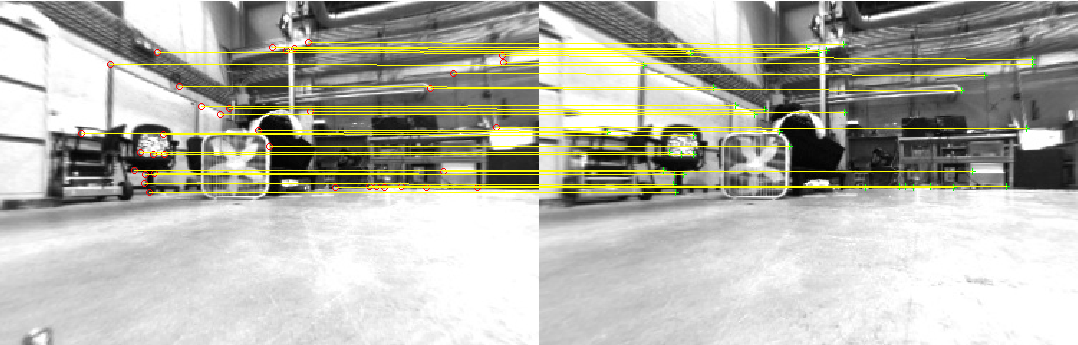
\includegraphics[width=450px]{feature.png}
		\label{feature}
	}

	\subfloat[Outliers removed (thick red circle) using RANSAC on reprojection errors.]{
		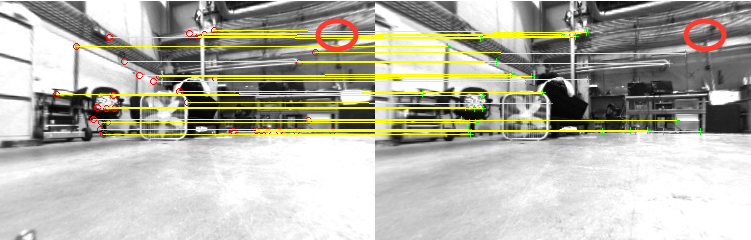
\includegraphics[width=450px]{featureoutlier.png}
		\label{featureoutlier}
	}
	\caption{Feature correspondences between \texttt{left000.jpg} and \texttt{right000.jpg} using a Harris feature detector.}
\end{figure}

\newpage

\item % c
Assuming a pinhole camera, triangulation of the stereo correspondences was performed using Direct Linear Transform (DLT) on the camera projection relationship, $x\times PX = 0$, where $P$ is the camera matrix, $X$ the 3-D world point, and $x$ the 2-D projection image point of $X$. The 3-D plots of the feature locations in Figure \ref{feature} is shown in Figure \ref{3d}.

\begin{figure}[h!]
	\centering
	\subfloat[Front view.]{
		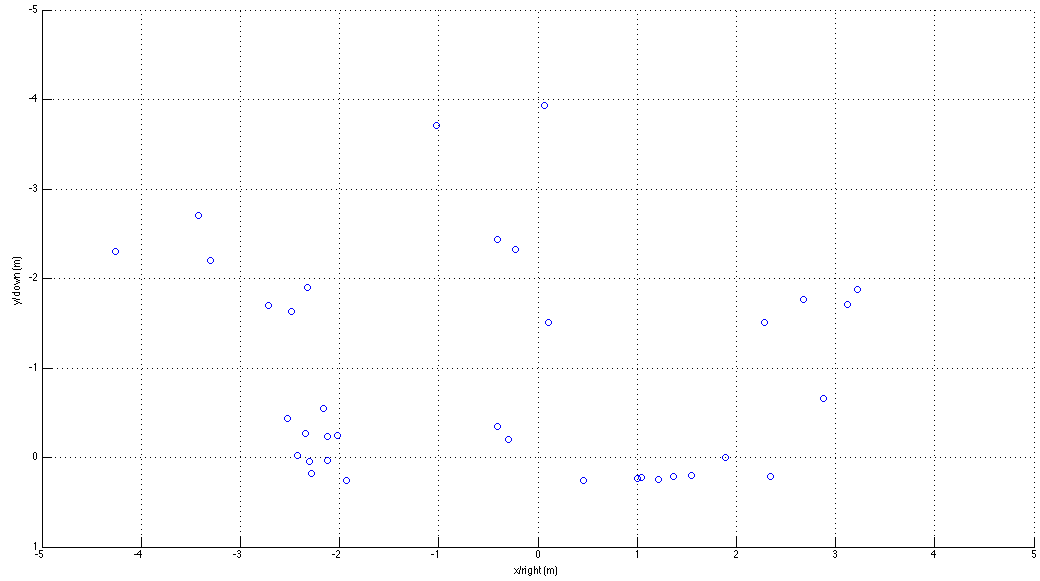
\includegraphics[height=170px]{3dfront.png}
	}
	
	\subfloat[Perspective view.]{
		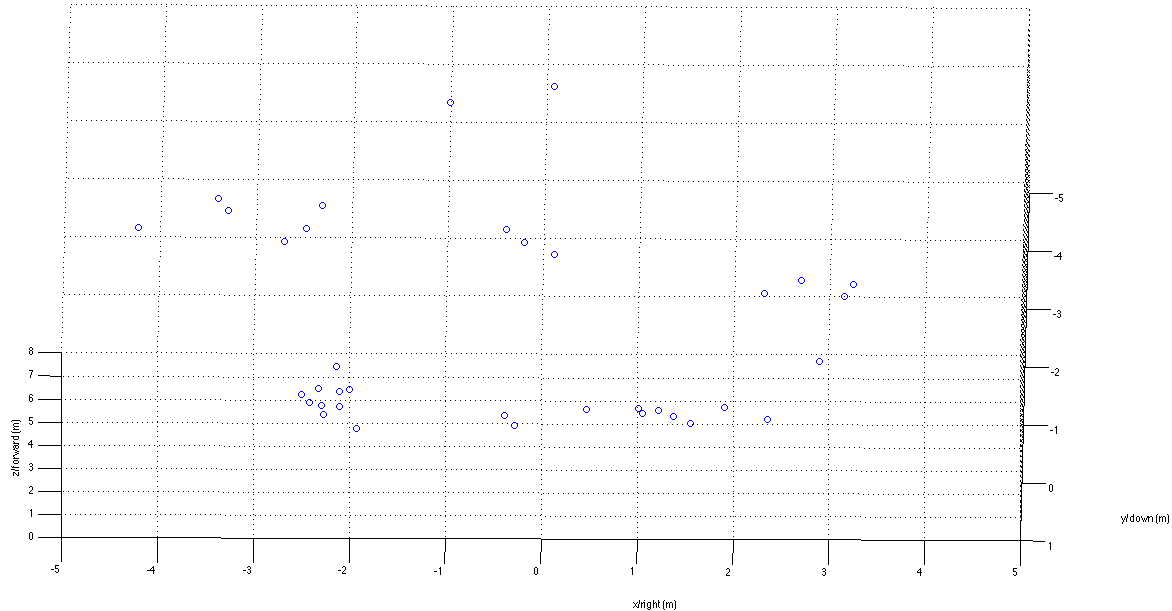
\includegraphics[height=170px]{3dperspective.png}
	}
	
	\subfloat[Top view.]{
		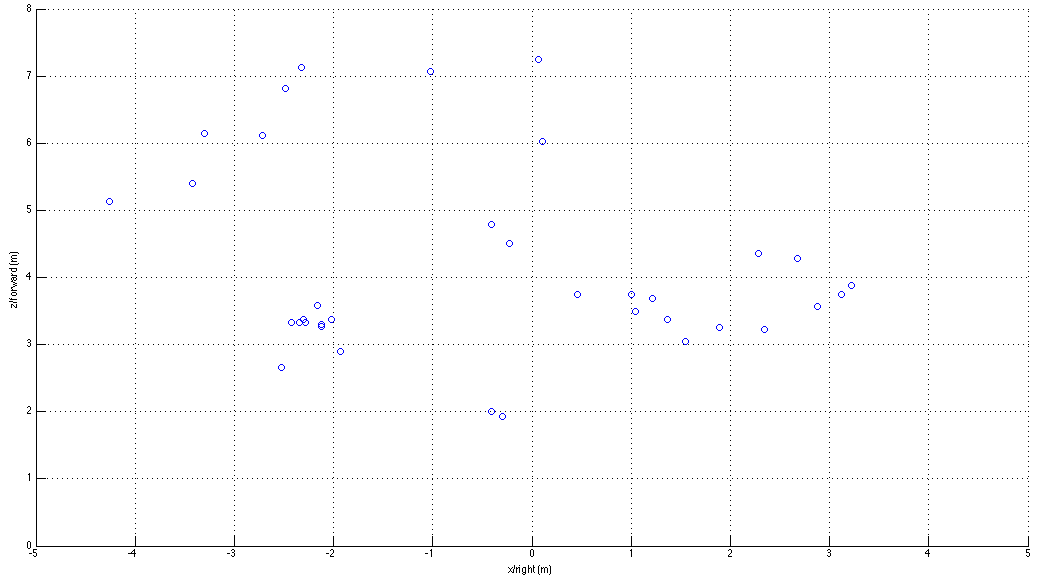
\includegraphics[height=170px]{3dtop.png}
	}
	\caption{The triangulated 3-D points of stereo correspondences.}
	\label{3d}
\end{figure}

\item % d
Correspondences between successive left images, \texttt{left000.jpg} and \texttt{left001.jpg} were found using the same feature detection and matching procedure described in parts (a) and (b).\\[12pt]
Let $x_n$ and $P_n$ be the correspondence points and the camera matrix for the nth image, then $x_1$ and the 3-D triangulated points, $X$, could be used to estimate the camera matrix, $P_1$ using the Direct Linear Transform. We assume the origin was at the camera center of the previous image, \texttt{left000.jpg} (i.e. $P_0 = K[I_3 | \textbf{0}_3]$, where $K$ is the 3-by-3 upper-triangular camera intrinsic matrix (identical for all images), $I_3$ the 3-by-3 identity matrix, and $\textbf{0}_3$ the 3-by-1 zero vector).\\[12pt]
To reject outlier correspondences, the competition of $P_n$ was wrapped within a RANSAC routine thresholded by the camera reproduction error, $e = || x_n - P_nX ||$. A minimum of 5.5 such correspondences was needed to compute the 11 degrees-of-freedom for the 3-by-4 camera matrix (12-1 dof for scale ambiguity). For convenience, six correspondences were used for every iteration of the RANSAC procedure. The inlier correspondences are shown in Figure \ref{featureoutlier}.\\[12pt]
For the computed camera matrix, $P_n$, the following relationship holds:
\begin{align*}
	P_n &= [P_{n, 1-3} | P_{n, 4}]\\
	&= K[R_n | t_n],
\end{align*}
where $R_n$ and $t_n$ are the incremental rotation and translation between camera frames $n-1$ and $n$. $P_{n, 1-3}$ was decomposed using RQ decomposition to obtain $K$ and $R_n$. Translation could be calculated using $t_n = K^{-1}P_{n, 4}$.

\item % e
Parts (a) to (d) were repeated to find $R_n$ and $t_n$ for every successive image pair. Assuming that the camera started at the origin of the world frame, a trajectory, shown in Figure \ref{traj}, was generated by composing sequential transformations of $R_n$ and $t_n$. Please note the frame convention aligns with that of the MATLAB image coordinates: x-right, y-down, z-forward. It is noticeable from Figure \ref{trajfront} that the end position falls below the starting position. This drift will be discussed in a later section. The position and orientation, in ZYX Euler angles, over time are shown in Figures \ref{pos} and \ref{orient}. To increase readability, the y values in all of the position plots in this document were negated due to a downward-pointing y-axis.

\begin{figure}[h!]
	\centering
	\subfloat[Front view.]{
		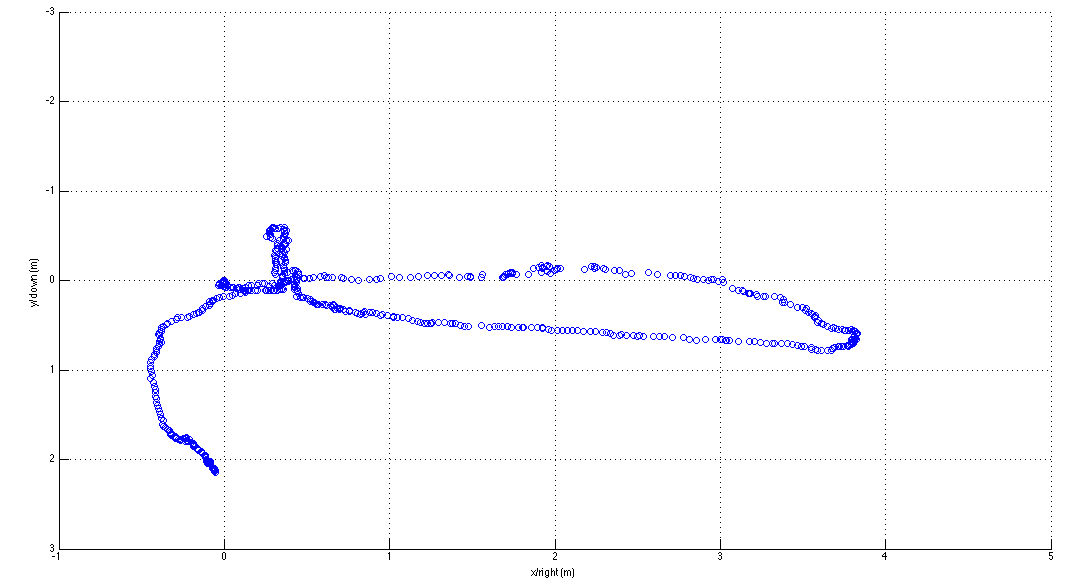
\includegraphics[height=160px]{trajside.png}
		\label{trajside}
	}
	
	\subfloat[Perspective view.]{
		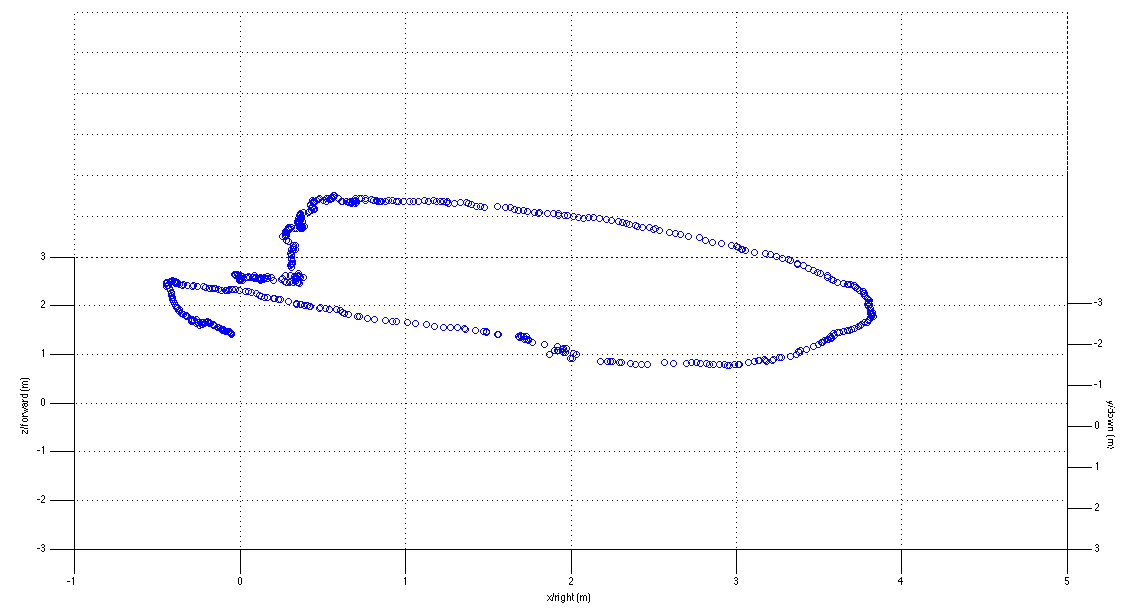
\includegraphics[height=160px]{trajperspective.png}
	}
	
	\subfloat[Top view.]{
		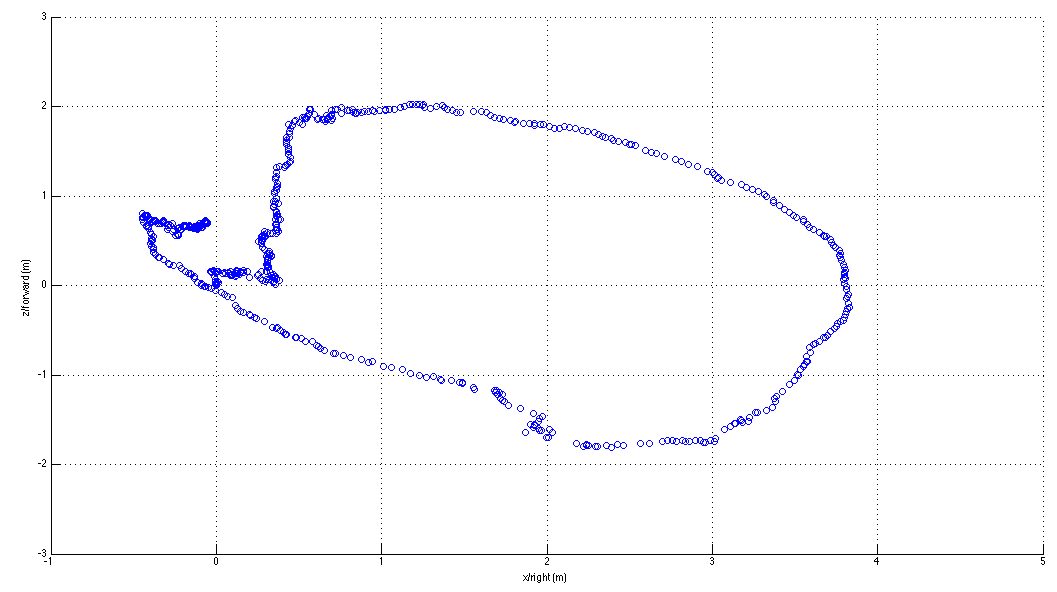
\includegraphics[height=160px]{trajtop.png}
		\label{trajtop}
	}
	\caption{The trajectory generated using incremental rotations and translations between successive images.}
	\label{traj}
\end{figure}

\begin{figure}[h!]
	\centering
	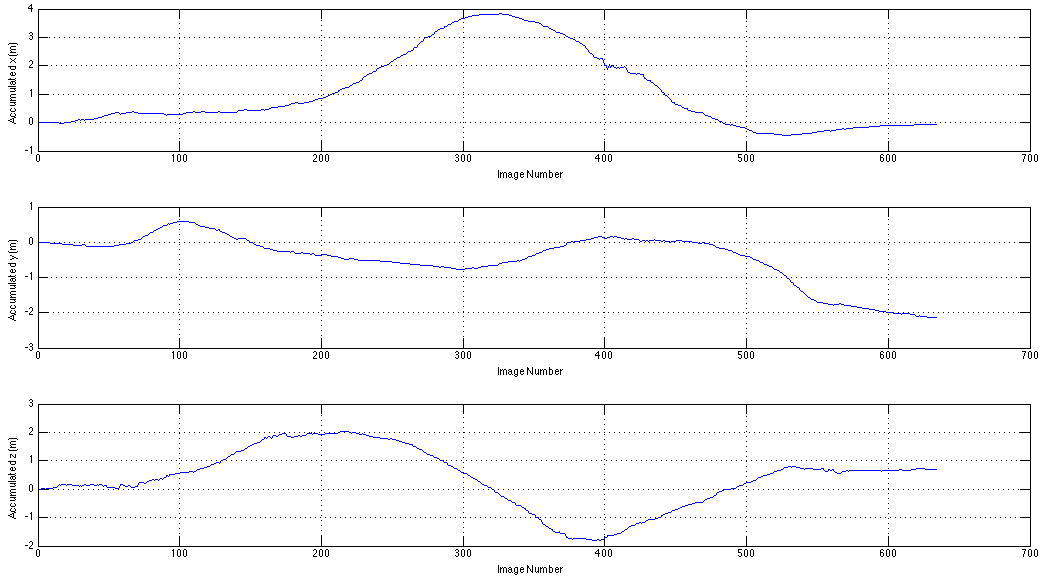
\includegraphics[width=450px]{position_adjusted.png}
	\caption{The accumulated position of the camera frame across all successive images.}
	\label{pos}
\end{figure}

\begin{figure}[h!]
	\centering
	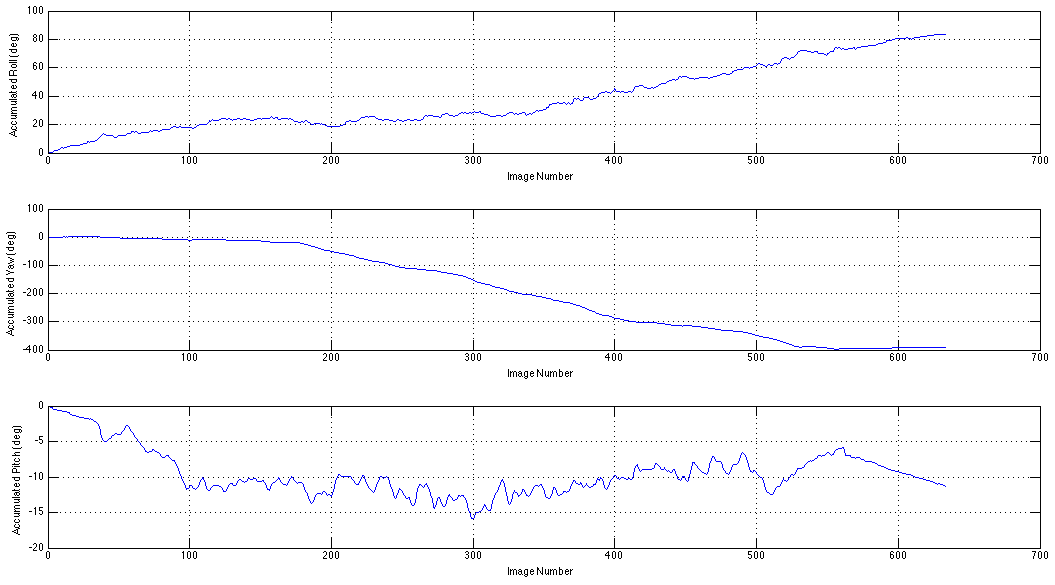
\includegraphics[width=450px]{orientation.png}
	\caption{The accumulated orientation (in ZYX Euler angles) of the camera frame across all successive images.}
	\label{orient}
\end{figure}

\item % f
Part (e) was repeated with different RANSAC iteration numbers and thresholds.
\begin{itemize}
\item Decrease the number of iterations by a factor of 10:\\
The trajectory is shown in Figure \ref{traj_iter} and the position and orientation plots are shown in Figures \ref{pos_iter} and \ref{orient_iter}. The decrease in the number of iterations resulted in additional drifts due to less optimal camera matrix estimations.

\begin{figure}[h!]
	\centering
	\subfloat[Front view.]{
		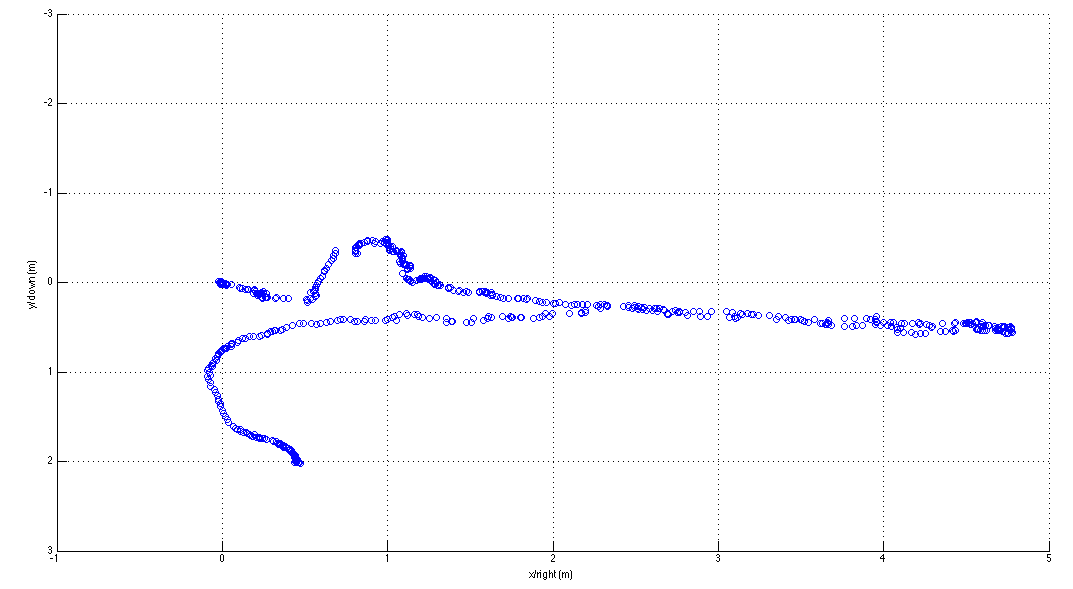
\includegraphics[height=160px]{trajside_iter.png}
	}
	
	\subfloat[Perspective view.]{
		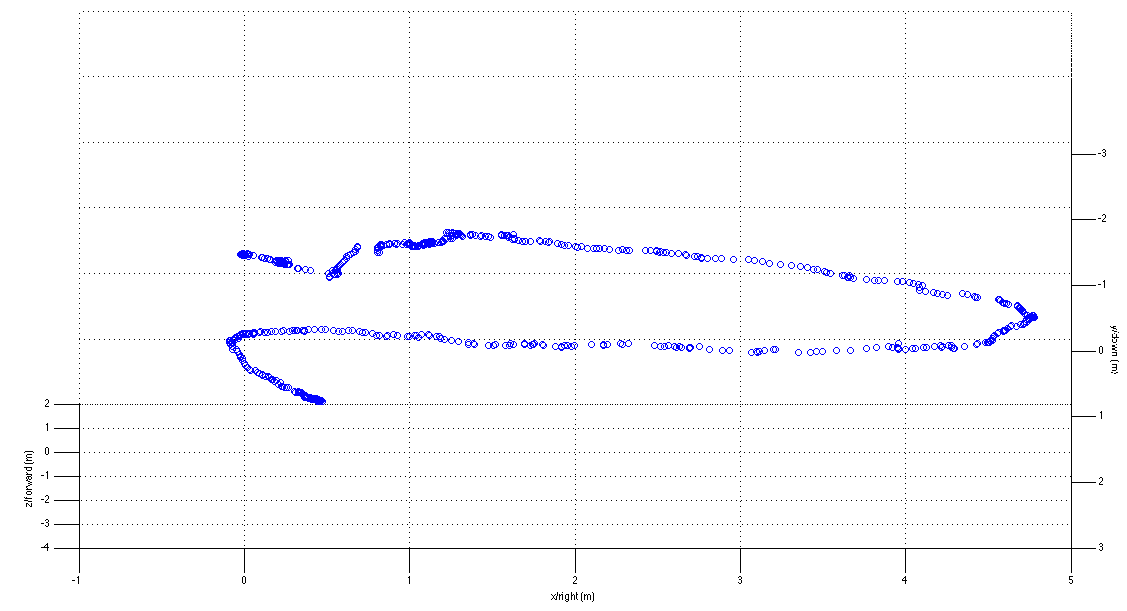
\includegraphics[height=160px]{trajperspective_iter.png}
	}
	
	\subfloat[Top view.]{
		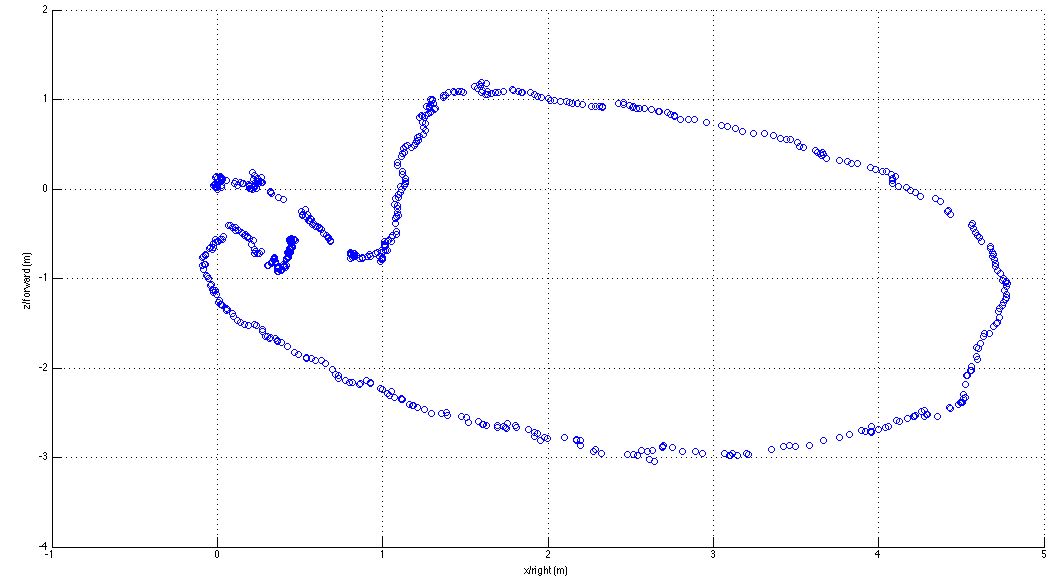
\includegraphics[height=160px]{trajtop_iter.png}
	}
	\caption{The trajectory generated using incremental rotations and translations between successive images for 10 times fewer RANSAC iterations.}
	\label{traj_iter}
\end{figure}

\begin{figure}[h!]
	\centering
	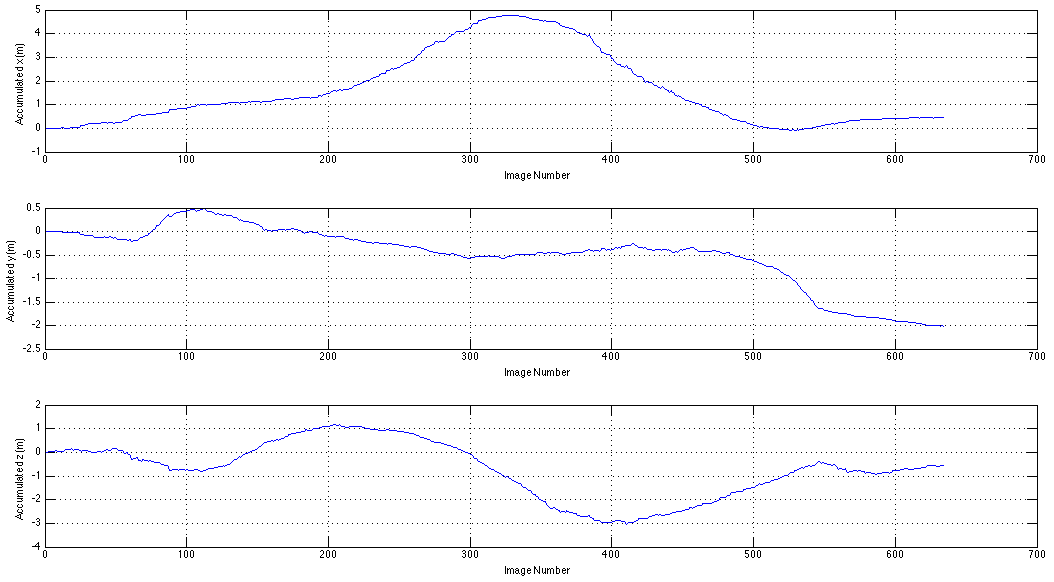
\includegraphics[width=450px]{position_adjusted_iter.png}
	\caption{The accumulated position of the camera frame across all successive images for 10 times fewer RANSAC iterations.}
	\label{pos_iter}
\end{figure}

\begin{figure}[h!]
	\centering
	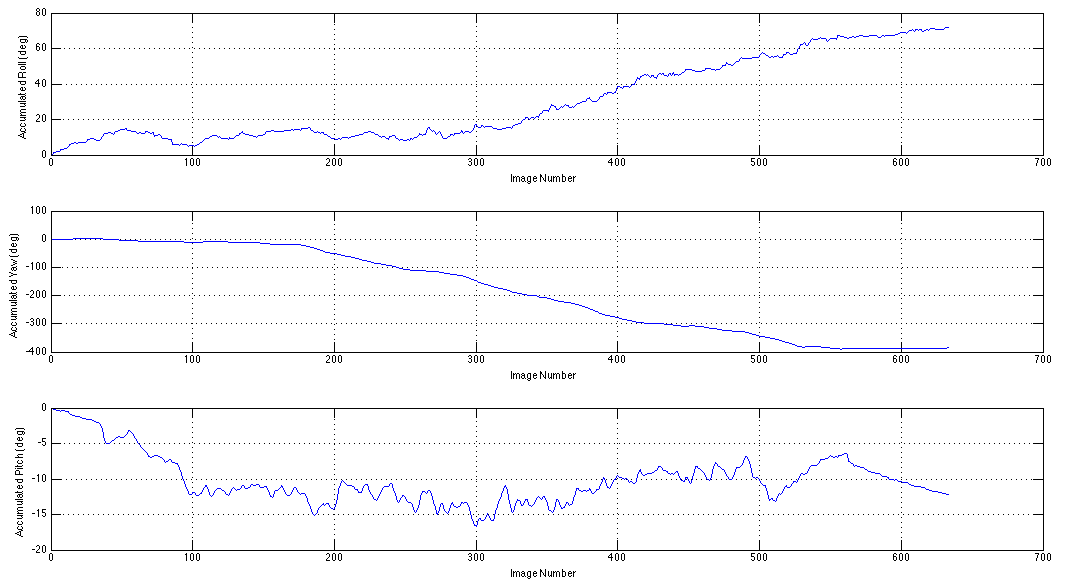
\includegraphics[width=450px]{orientation_iter.png}
	\caption{The accumulated orientation (in ZYX Euler angles) of the camera frame across all successive images for 10 times fewer RANSAC iterations.}
	\label{orient_iter}
\end{figure}

\item Increase the threshold by a factor of 10:\\
The trajectory is shown in Figure \ref{traj_thres} and the position and orientation plots are shown in Figures \ref{pos_thres} and \ref{orient_thres}. A larger threshold potentially allowed outliers to be included as inliers during the RANSAC routine, thus yielding less optimal and noisier camera matrix estimations. As a result, additional errors in drift were introduced to the trajectory.

\begin{figure}[h!]
	\centering
	\subfloat[Front view.]{
		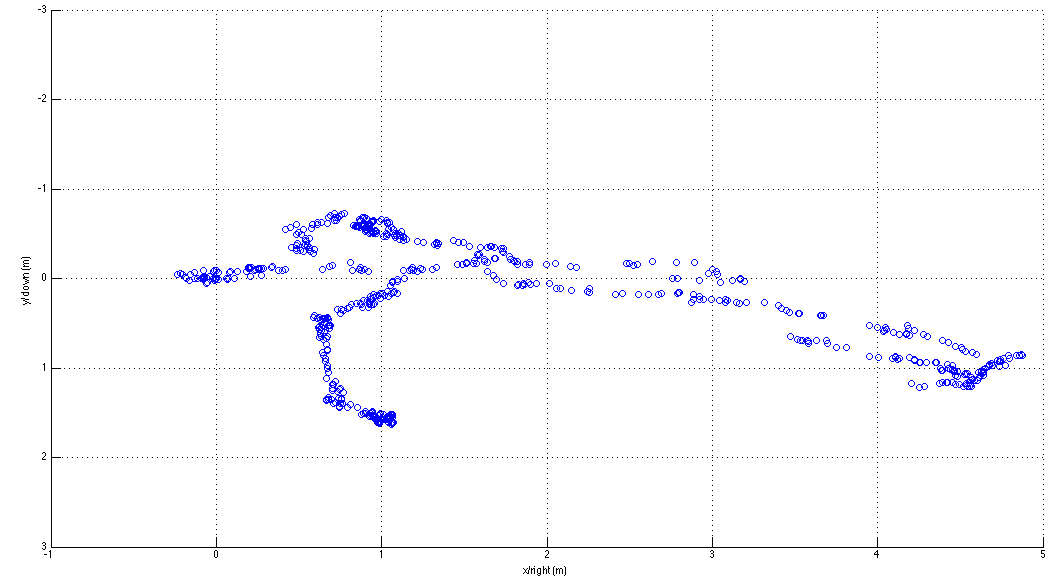
\includegraphics[height=160px]{trajside_thres.png}
	}
	
	\subfloat[Perspective view.]{
		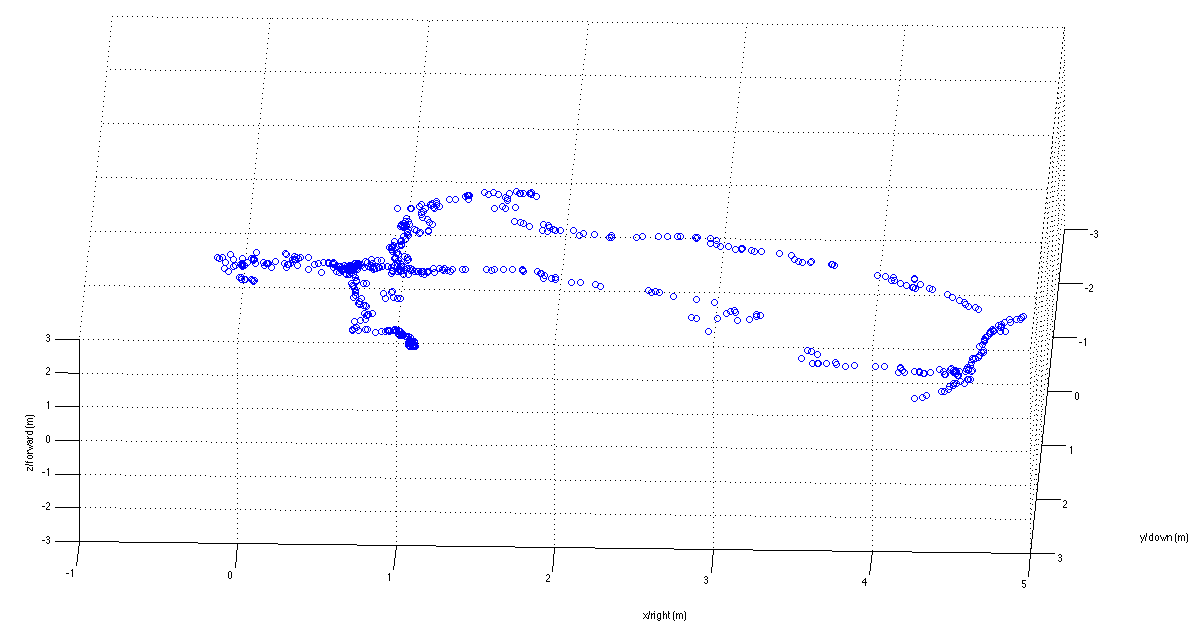
\includegraphics[height=160px]{trajperspective_thres.png}
	}
	
	\subfloat[Top view.]{
		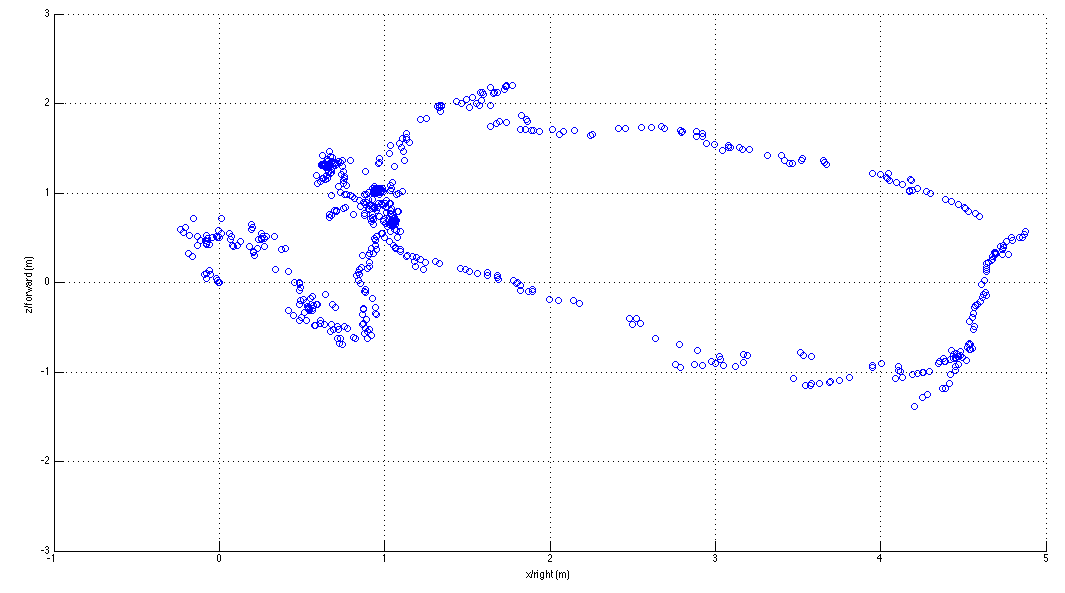
\includegraphics[height=160px]{trajtop_thres.png}
	}
	\caption{The trajectory generated using incremental rotations and translations between successive images for 10 times RANSAC threshold.}
	\label{traj_thres}
\end{figure}

\begin{figure}[h!]
	\centering
	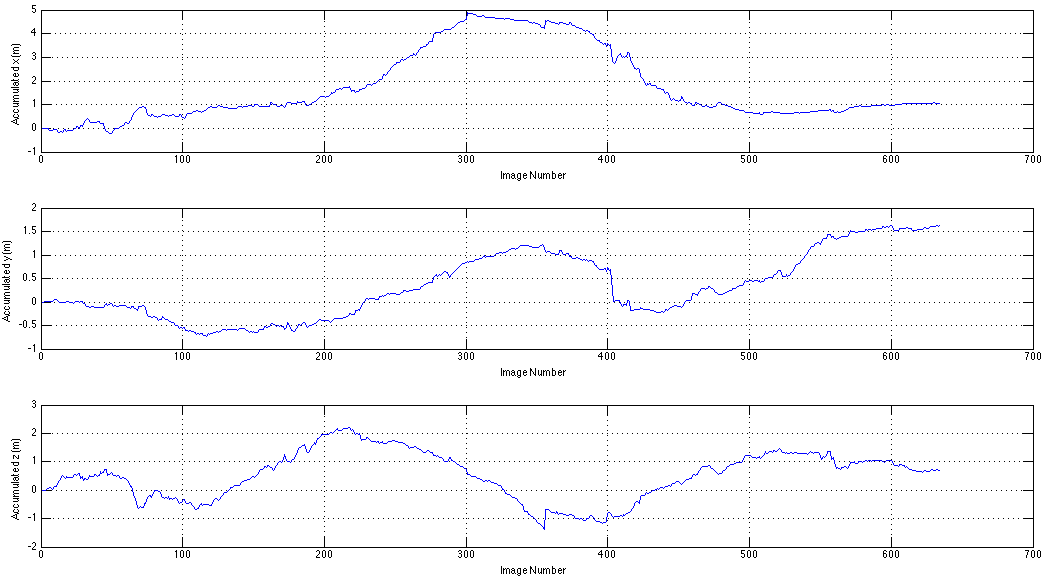
\includegraphics[width=450px]{position_adjusted_thres.png}
	\caption{The accumulated position of the camera frame across all successive images for 10 times RANSAC threshold.}
	\label{pos_thres}
\end{figure}

\begin{figure}[h!]
	\centering
	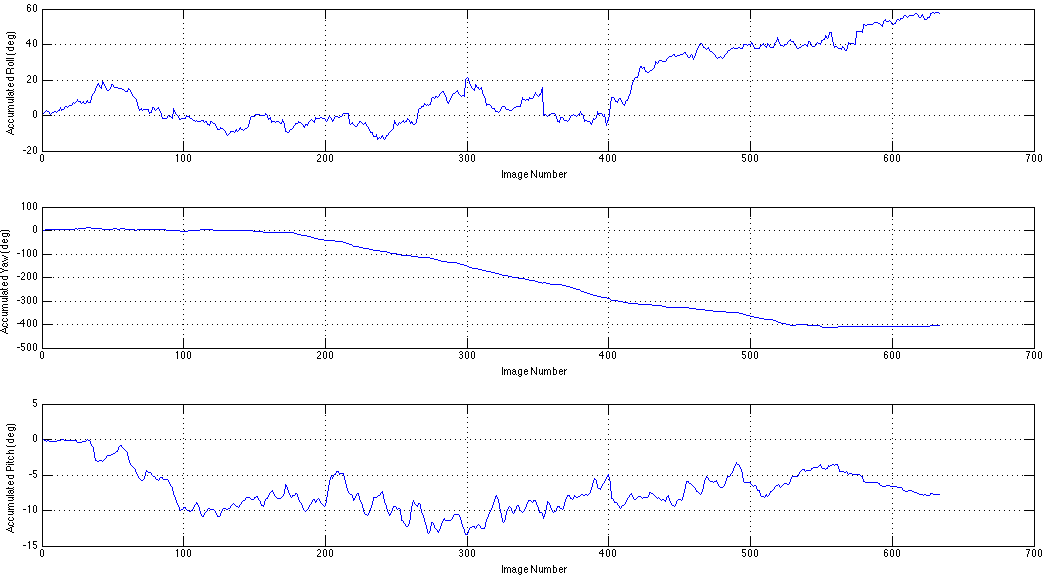
\includegraphics[width=450px]{orientation_thres.png}
	\caption{The accumulated orientation (in ZYX Euler angles) of the camera frame across all successive images for 10 times RANSAC threshold.}
	\label{orient_thres}
\end{figure}

\end{itemize}

\newpage

\item % g
The trajectory computed did not return exactly to the starting position (see Figure \ref{trajtop}). As seen in Figure \ref{trajside}, the height of the final position was even below ground level. This drift could be explained by the accumulated errors in estimations across each pair of successive frames. After hundreds of estimations, the errors became observably significant in the position estimates. Figures \ref{pos_drift} and \ref{orient_drift} display the "drift profile" in position and orientation obtained by calculating the estimation errors between each image frame and its own.\\[12pt]
Knowing that such drift was proportional to the image frames calculated, a new trajectory was generated using only every seven frames, as shown in Figure \ref{traj_int7}. The position and orientation are shown in Figure \ref{pos_int7} and \ref{orient_int7}. This interval of seven images was determined empirically. Intuitively, a smaller interval would account for more image drifts while a larger interval would start to exhibit unstable estimations due to drastic scene (and hence, features) changes.

\newpage

\begin{figure}[h!]
	\centering
	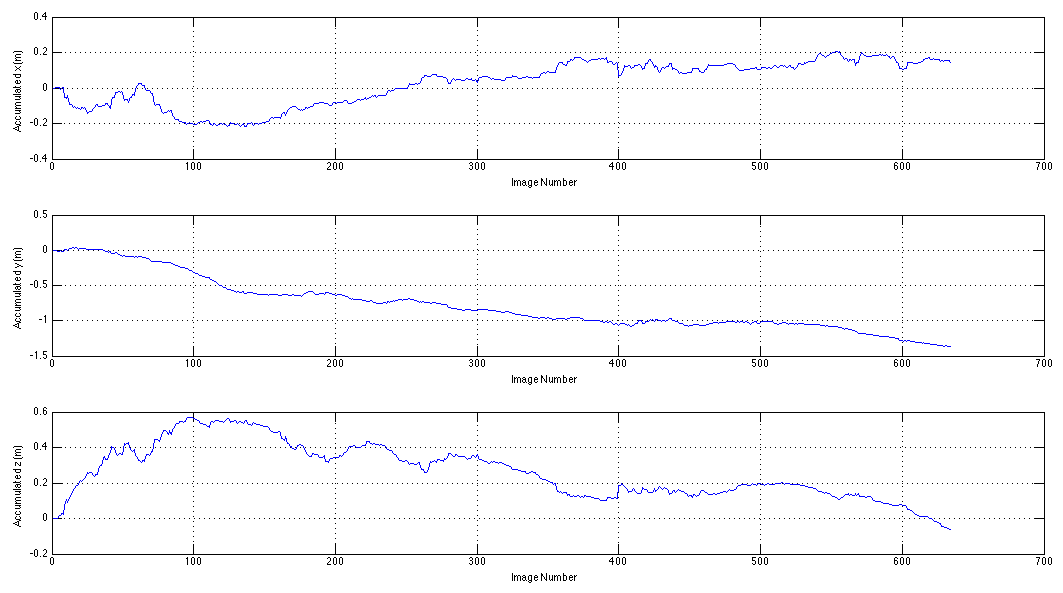
\includegraphics[width=450px]{position_drift.png}
	\caption{The accumulated position drift of the camera frame across all successive images.}
	\label{pos_drift}
\end{figure}

\begin{figure}[h!]
	\centering
	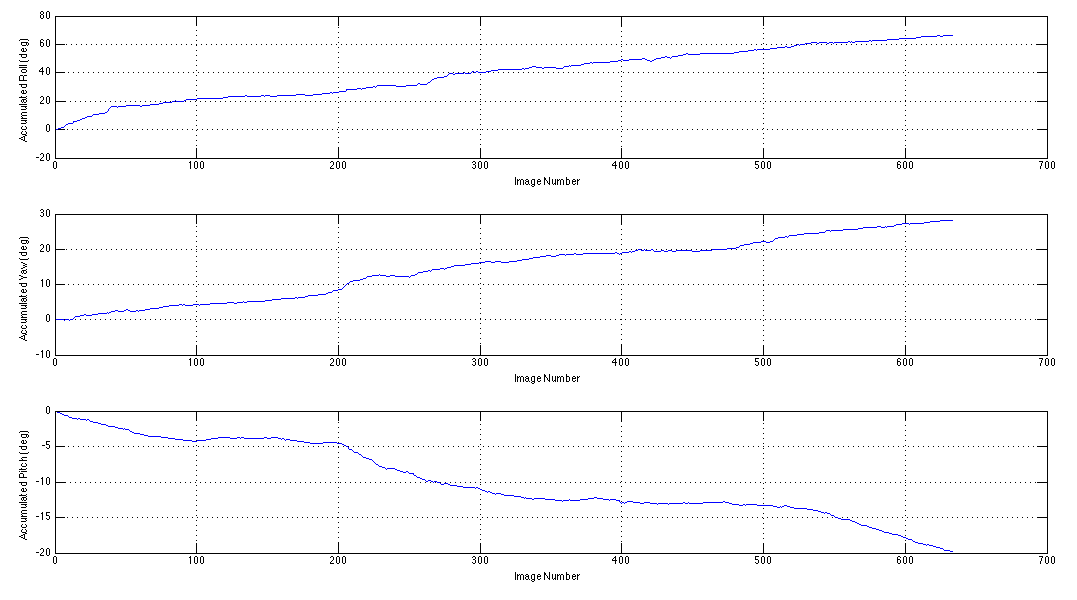
\includegraphics[width=450px]{orientation_drift.png}
	\caption{The accumulated orientation (in ZYX Euler angles) drift of the camera frame across all successive images.}
	\label{orient_drift}
\end{figure}

\begin{figure}[h!]
	\centering
	\subfloat[Front view.]{
		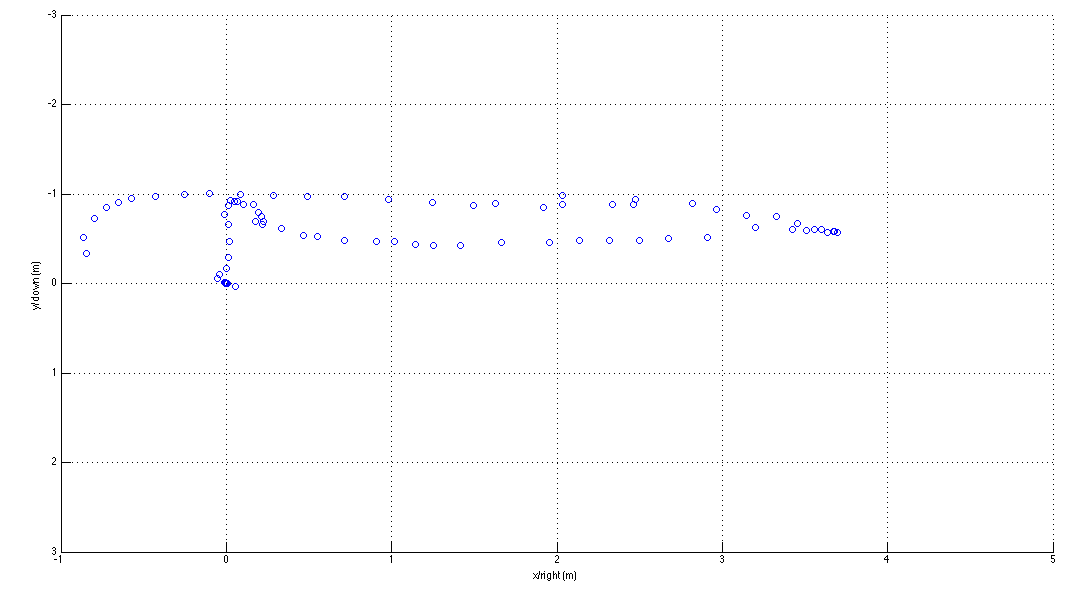
\includegraphics[height=160px]{trajside_int7.png}
	}
	
	\subfloat[Perspective view.]{
		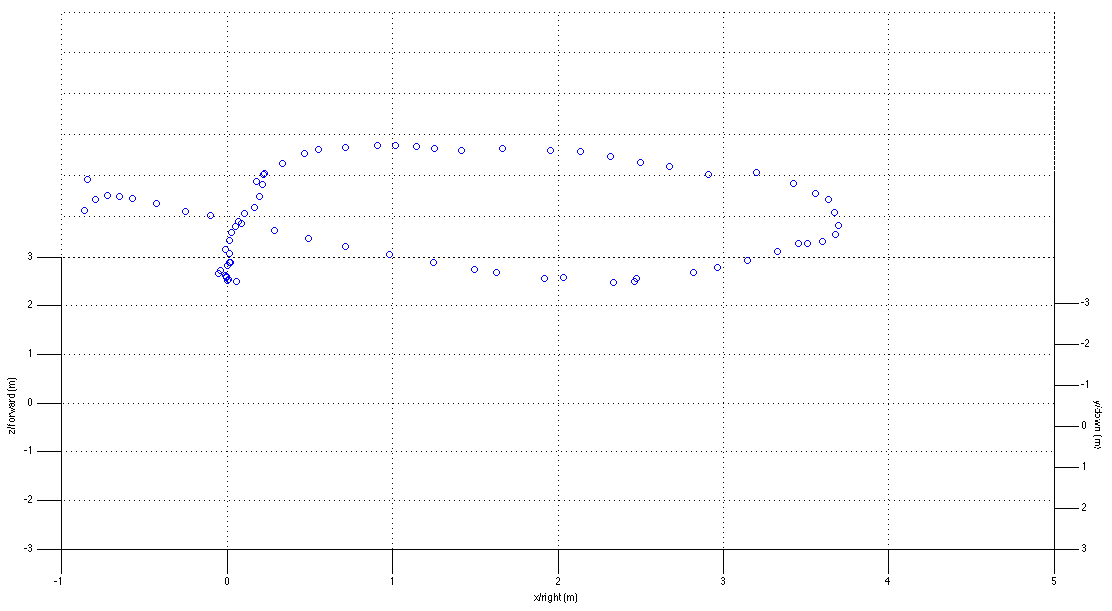
\includegraphics[height=160px]{trajperspective_int7.png}
	}
	
	\subfloat[Top view.]{
		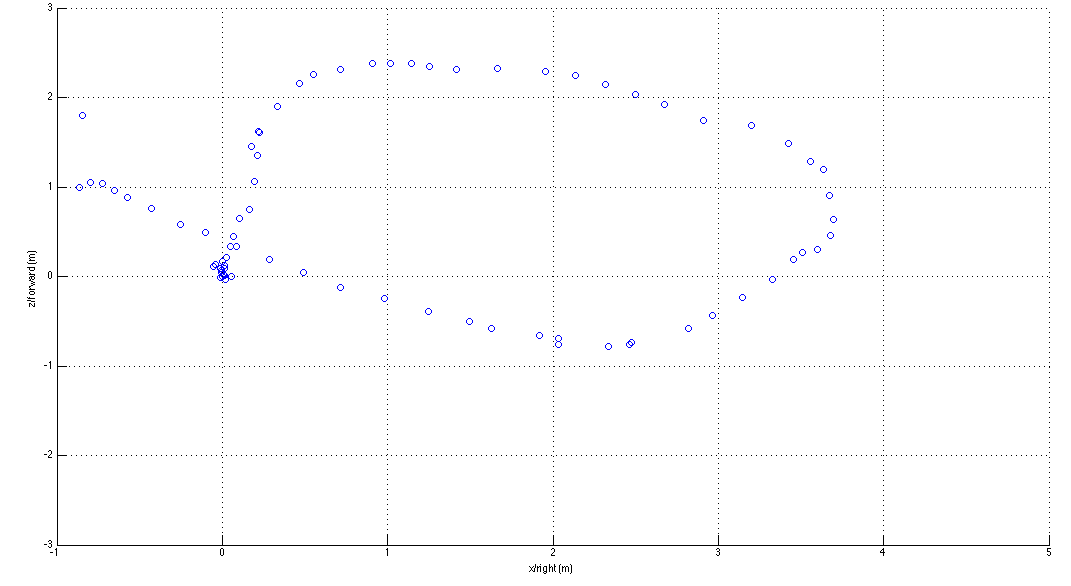
\includegraphics[height=160px]{trajtop_int7.png}
	}
	\caption{The trajectory generated using incremental rotations and translations between every seven images.}
	\label{traj_int7}
\end{figure}

\begin{figure}[h!]
	\centering
	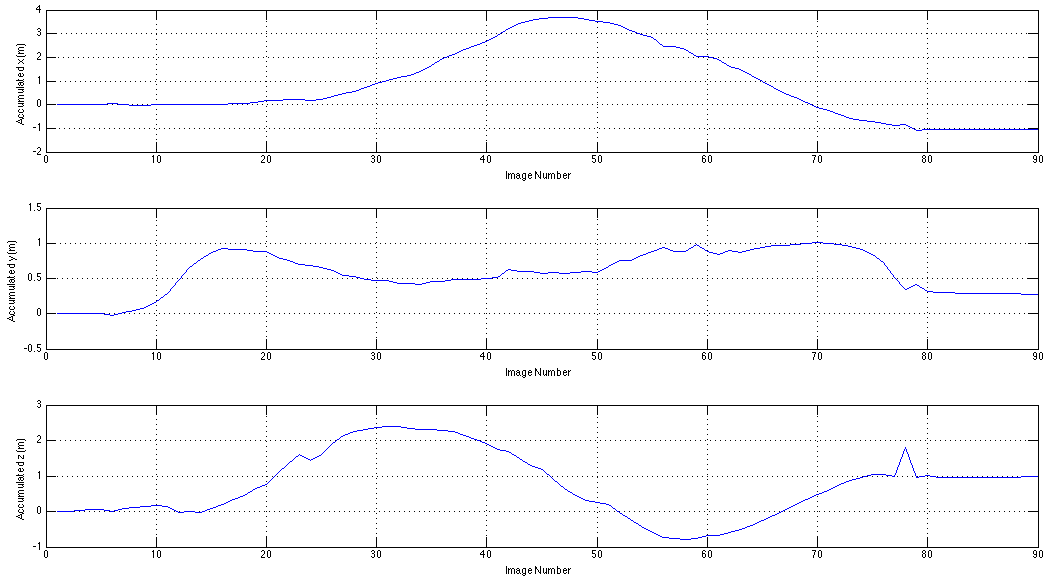
\includegraphics[width=450px]{position_adjusted_int7.png}
	\caption{The accumulated position of the camera frame between every seven images.}
	\label{pos_int7}
\end{figure}

\begin{figure}[h!]
	\centering
	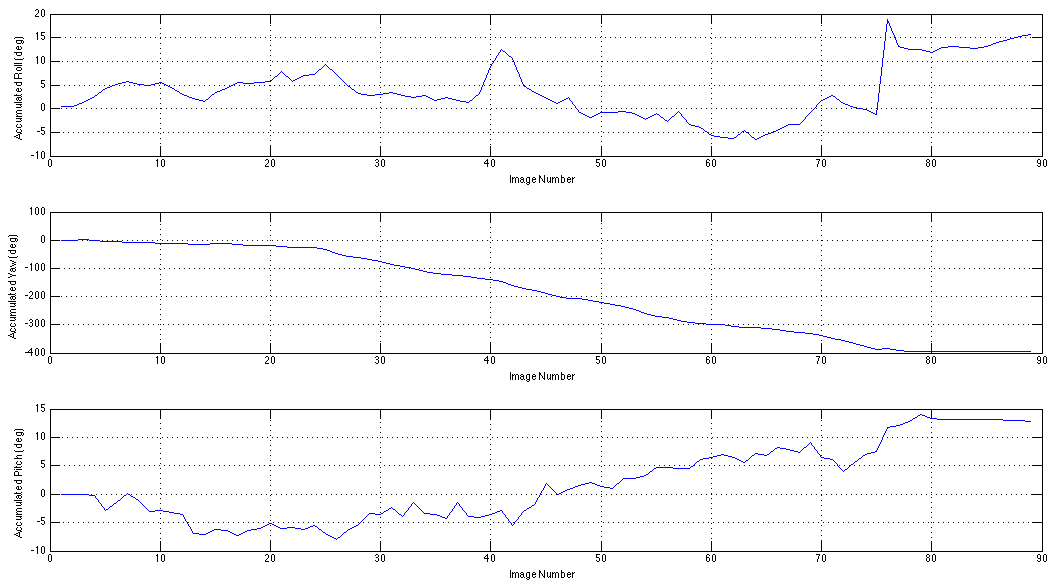
\includegraphics[width=450px]{orientation_int7.png}
	\caption{The accumulated orientation (in ZYX Euler angles) of the camera frame between every seven images.}
	\label{orient_int7}
\end{figure}

\end{enumerate}


\end{document}

%%%%%%%%%%%%%%%%%%%%%%%%%%%%%%%%%
% Elements 

\begin{comment}

% Equations
\begin{align}
	H &=
	\begin{bmatrix}
		X\\ Y\\ Z\\ 1
	\end{bmatrix}
\end{align}

% Figure/Subfitures
\begin{figure}[h!]
	\centering
	\includegraphics[width=350px]{xxx.jpg}
	\caption{caption}
	\label{label}
\end{figure}

\begin{figure}[h!]
	\centering
	\subfloat[subcaption1]{%
		\includegraphics[height=150px]{xxx.jpg}
	}
	\subfloat[subcaption2]{%
		\includegraphics[height=150px]{yyy.jpg}
	}
	% An empty line here makes a second row
	\subfloat[subcaption3]{%
		\includegraphics[height=150px]{zzz.jpg}
	}
	\caption{caption}
	\label{label}
\end{figure}

% Tables/subtables
\begin{table}
	\centering
	\subfloat[subcaption1]{
		\begin{tabular}{ | c | c | c | c | }
			\hline
			\  & \multicolumn{3}{ |c| }{Out} \\ \hline
			\multirow{3}{*}{Truths} & X & 0 & 1 \\ \cline{2-4}
			& 0 & 71.75\% & 3.52\% \\ \cline{2-4}
			& 1 & 3.23\% & 21.50\% \\ \hline
		\end{tabular}
	}\hspace{50px}
	\subfloat[subcaption2]{
		\begin{tabular}{ | c | c | c | c | }
			\hline
			\  & \multicolumn{3}{ |c| }{Out} \\ \hline
			\multirow{3}{*}{Truths} & X & 0 & 1 \\ \cline{2-4}
			& 0 & 45.76\% & 21.61\% \\ \cline{2-4}
			& 1 & 5.83\% & 26.8\% \\ \hline
		\end{tabular}
	}
	% An empty line here makes a second row
	\subfloat[subcaption]{
		\begin{tabular}{ | c | c | c | c | }
			\hline
			\  & \multicolumn{3}{ |c| }{Out} \\ \hline
			\multirow{3}{*}{Truths} & X & 0 & 1 \\ \cline{2-4}
			& 0 & 71.43\% & 3.83\% \\ \cline{2-4}
			& 1 & 13.45\% & 11.28\% \\ \hline
		\end{tabular}	}\hspace{50px}
	\subfloat[subcaption]{
		\begin{tabular}{ | c | c | c | c | }
			\hline
			\  & \multicolumn{3}{ |c| }{Out} \\ \hline
			\multirow{3}{*}{Truths} & X & 0 & 1 \\ \cline{2-4}
			& 0 & 52.37\% & 14.99\% \\ \cline{2-4}
			& 1 & 14.88\% & 17.76\% \\ \hline
		\end{tabular}
	}
	\caption{table caption}
\end{table}

% Lists
\begin{enumerate}[label=\alph*)]
	\item item1
	\item item2
	\item item3
\end{enumerate}

% Vertical space
\vspace{20px}

\end{comment}
